\documentclass[12pt,a4paper,oneside]{article}
\usepackage{ctex,graphicx,setspace}
\setstretch{1.25}

\title{人工智能导论报告}
\author{陈海弘 23354049}
\date{2024.5.10}

\begin{document}


\maketitle

\newpage
\tableofcontents
\section{课程内容概述}
\subsection{人工智能导论前沿技术}
\subsubsection{人工智能概论}
何谓人工智能?计算机科学加上智能表现所构成的环境交互,也就是制造具有智能表现的机器,能够与环境交互并努力实现目标, 就是人工智能。
为了实现这个交互,机器需要具有感知,识别,认知,推理,判断,预测,学习,行为的能力。

人工智能的定义有三个层面。
在广义下的定义是,通过计算机实现人的头脑思维所产生的效果,对能够从环境中获得感知并执行行动的智能体的描述和建构。
产业上的定义是,构建包括数据、计算引擎、算法、技术、基于人工智能算法和技术进行研发及拓展应用的企业。
技术上的定义是,人类在利用和改造机器的过程中所掌握的物质方法,手段,知识等各种活动的总和。
总的来说,就是通过机器实现人的头脑思维,使其具备感知、决策和行动力。

人工智能的三大核心:算力、算法、数据。

人工智能对于数据的需求多样性,导致需求大量且高质量的数据。当有了大量数据后,需要高端的处理器、芯片来进行运算,而运算的速度又取决于算法,算法越精确,鲁棒性越来越好,人工智能才能越来越强大。
算力决定于GPU、CPU等等硬件,算法决定于深度学习,机器学习,也就是算法的精确性,数据决定于数据库,结构化等。
\subsubsection{人工智能主要技术分支}
通讯、感知和行动是现代人工智能的三个关键能力,基于此,可以将其分为四个技术分支,计算机视觉(CV),自然语言处理(NLP),计算机听觉(CA)和智能机器人。

计算机视觉要解决的问题就是看懂图像里的内容。其分布之广,技术之成熟,自始至终都是最热门的行业之一。
图像分类网络的发展经历了LeNet、AlexNet、VGG、GoogLeNet、ResNet,DenseNet,EfficentNet等等。

自然语言处理是指用计算机来处理,理解以及运用人类语言,实现人机交流的目的。其实际运用有,机器翻译,问答,对话,文本摘要,阅读理解,文本生成等等。

而计算机听觉是仅次于视觉的重要通道,目前大量基于计算机听觉的技术应用已经出现在人们的生活中,比如Siri,音乐识别,语音识别,语音合成,语音分离等等。

最后的智能机器人的关键技术在于路径规划,人机接口,机器人视觉,多传感信息融合,智能控制,导航和定位这六点。
\subsubsection{典型新型智能机器人}
从电影中的钢铁侠出现在生活中,到元宇宙,机器人虚拟映射远程操控系统,还有无感交互——普适机器人体系,智能机器人正在蓬勃发展。
\subsubsection{前沿应用与案例}
自动驾驶车,AR,智能眼镜,问答机器人,手术机器人,无人机,等等应用,其遍布之广,让我相信未来人工智能的应用大有可为。
\subsection{自然语言处理}
人工智能是怎么实现的?最主要的就是自然语言处理。自然语言处理是人工智能的一个重要分支,是人工智能的基础。
自然语言处理可以可以定义为研究在人与人交际中以及在人与计算机交际中的语言问题的一门学科。它要研制表示语言能力,语言应用的模型,通过建立计算框架来实现这样的语言模型,提出相应的方法来不断完善这样的语言模型,
根据这样的语言模型设计各种实用系统,探讨这些应用系统的评测技术。

自然语言处理起源于文本分类、文本聚类和内容生成等单项技术。
文本聚类的目的是将给定的文本集合划分成不同的类别。文本聚类和文本分类的根本区别在于:分类事先知道有多少个类别,而聚类则事先不知道有多少个类别。
内容生成也有很多类型,可以分为文本缩写,文本改写,文本扩写等等。

自然语言处理还可以实现信息抽取,包括命名实体识别、实体消歧、关系抽取和事件抽取。除了信息抽取之外,它还可以作为推荐系统,在智能网联汽车大力发展的当下,将出现一个市场体量巨大的车内媒体生态。

自然语言处理技术在国民经济、社会管理、信息服务和国家安全等各个领域中都有非常重要的应用,市场需求巨大。

\subsection{人工智能汽车}
汽车智能化、网联化时代已然到来。
\subsubsection{车联网和ICV的由来}
智能网联汽车从哪里来?

物联网的产生是在经济危机下的推动发生的,全球性的经济危机是科技创新的动力,但科技创新的进步并不一定要发生经济危机。
随着传感技术的成熟,例如图像处理技术,网络接入和信息处理能力大幅提高,也就是基于海量信息收集和分类处理的能力大大提高,物联网诞生了。

物联网就是利用条码、射频识别(RFID)、视频、全球定位系统、激光扫描器等信息传感设备,
按约定的协议,实现人与人、人与物、物与物的在任何时间、任何地点的连接
(Anything、Anytime、Anywhere),从而进行信息交换和通讯,以实现智能化识别、
定位、跟踪、监控和管理的庞大网络系统。


而车联网就是把物联网的方法和技术应用到汽
车交通行业,就是车联网,车联
网是物联网的一个典型行业应用,
智能网联汽车是车联网的重要载体。

在AI+产业中,物联网对社会发展作出了巨大的贡献。智能物流,流通环节节能,智能家居,智能农业等等。

所以总而言之,智能网联汽车是车联网的重要载体,车联网只是物联网的一个典型行业应用,而物联网是新一代信息理论和技术的组成,新一代信息技术的推手之一是经济危机。

究其根本,物联网和人工智能的关系是,物联网是人工智能的一个重要载体,人工智能是物联网的一个重要技术支撑。物联网就像GPU,人工智能就像算法软件。
同时,人工智能为物联网面临的数据难题提供了最好的解决方案,人工智能的分析方法可以引入进来。
人工智能和物联网相互融合,利用人工智能实时分析数据的物联网设备端正走入我们。
\subsubsection{智能网联汽车的定义}
什么是智能网联汽车?

网联车,是通过GPS、摄像头图像处理、RFID等各类传感装置,车辆可以
完成自身环境和状态信息的采集;通过互联网、移动通信技术,所有车辆
可以将自身的各种信息传输汇聚到中央处理器;通过计算机技术,大
量车辆的信息可以被分析和处理,从而实现汽车的网联化。

在互联网时代的互联,就是每个事物都带有IP,而物联网时代的车联网,就是每个汽车都带有感知器,存储信息标签进入网络空间。

而智能车,主要围绕的是单一车辆(一
般称为单车智能),或者说智能汽车主要指的是围绕转向、驱动、制动的自
主控制/辅助控制/辅助驾驶。

简单来说,网联车和智能汽车的区别是,智能汽车必须对汽车三
个基础控制要素发生控制关系,就是说不仅仅是数据交互,且有对汽车三
个基础控制要素的伺服控制或间接产生伺服控制。否则,只能算网联化。

前文所提到的智能网联汽车(ICV),是指网联
车与智能车的有机联合,搭载先进的车载传感器、控制器、执行器等装
置,并融合现代通信与网络技术,实现车与“人、车、路、环境、云”
等智能化的信息交换共享,目的是完成安全、节能、环保、高效、便携
的行驶,并最终可部分替代或完全替代人来操作的新一代汽车。
\subsubsection{自动驾驶试验的步骤}
自动驾驶试验的步骤主要分为六步。

第一步,自动驾驶车辆直线导航试验。在此之前,需要做车辆转向系统、驱动系统、制动系统的系统辨识试验。

第二步:自动驾驶车辆有干扰的直线导航试验,也就是自主导航控制器作用。

第三步:自动驾驶车辆的弧线导航试验,现在可以利用当前人工智能的优势去克服“难建模、非线性、时变特性”等问题。

第四步:自动驾驶车辆的校园综合试验,人工智能现在对复杂场景变化有较高的自适应性,比如半阴半阳、上下坡、不同天气等。

第五步:自动驾驶车辆的户外综合性试验演示。国内有早期的区域交通智能车辆,国外有NTU的机器人等研究所。所谓人工智能时代,就是现在所推崇的“功能性智能车辆、低速自动驾驶车辆”。

第六步:多无人车/本质也可以说是多机器人的户外协同控制试验演示。早期的多智能车辆协同避碰试验,亮点在于高精度定位、精确的伺服控制
早期提出无人车Real Time Maps概念、Intersection-Safe 的网联概念。

现在,智能网联汽车分为L0-L5,目前世面上的自动驾驶车辆大多数是L2-L3,L4-L5的车辆还在研究中。
\subsubsection{自动驾驶车辆的分布}
据自动驾驶实践特点,
一般有五类:“区域交通智能车辆、智能网联卡车、智能轿车、自动
物流运输小车、轮式移动机器人”。

而主要考虑这几个方面,人、环境、路线、气候、时间。人群是多还是少?是否约束人?
环境是否可知?能否适用大多数情况,遍历性?
路线是否固定?是否单一?是否具有遍历性?
气候是春夏秋冬哪一个?是否有雨雪等恶劣天气?
时间是否固定?还是24小时全天候?依据这几个方向去考虑自动驾驶,就可以得到一个较好的结果。

无人车的理论和实践,敬重人性、大自然最为重要。只有符合人、大自然的规律,才可以更好的让无人车融入生活。

自动驾驶车辆不等于私家车就可以城市道路上完全自主驾驶,自动驾驶技术的应用主要还
是区域交通智能车辆,智能卡车重点
是网联和标准,而智能轿车是辅助驾驶。
\subsection{智能机器人}
\subsubsection{特种机器人无人机}
无人驾驶航空器(UA)是一架由遥控站管理
包括远程操外或自主飞行)的航空器,也称遥控驾驶航空器
Piloted Aircraft),以下简称无人机。
无人机发展迅速,西方国家一直处于领先地位。

其可以按照用途来分类,分为军用无人机,民用无人机。目前超过70\%的无人机用作军事用途。
无人飞行器可以大致分为六种,固定翼、旋翼、多旋翼、无人飞艇、伞翼、扑翼。

系统组成为飞行器,控制站,通信链路三个部分。飞行器主要考虑动力系统,机载核心系统,任务载荷。控制站也就是无人机地面站,不同功能的控制站通过通信设备连接,构成无人机地面站系统。
通讯链路分为机载终端和天线、地面终端和天线、通信链路三个部分。

总而言之,无人机有优缺点,但只要解决了长续航、轻自重、大负载、抗通讯干扰等问题,未来无人机的应用前景是非常广阔的。
\subsubsection{特种机器人水下}
机器人就是靠着自身动力和控制能力来实现各种功能的一种机器。是一种可以编程和
多功能的操作机;或者是为了执行不同任务而具有可用电脑改变和可编程动作的专门系统。

其中,阿西莫夫提出的机器人三大法则一直为后世机器人的创作提供指导意义。机器人不得伤害人类,或者目睹人类个体将遭受危险而袖手不管;
机器人必须服从人给予它的命令,当该命令与第一定律冲突时例外;
机器人在不违反第一、第二定律的情况下要尽可能保护自己的生存。

同样的,机器人也分为工业机器人,和特种机器人。工业机器人就是面向工业领域的多关节机械手或多自由度机器人。特种机器人就是除了工业机器人之外,用于非制造业并且服务于人类的各种先进机器人。其中,特种机器人可以分为军用机器人,水下、农用机器人等等。

但是如果不考虑使用目的,仅考虑工作环境,特种机器人的核心分类是空中、水面、水下和陆地机器人。环境对机器人的物理形态、设计形式、主要零部件有较大影响,这也是特种机器人要解决的核心问题。

而评价一个机器人的能力,标准包括,智能,也就是感觉和感知;机能,指变通性、通用性和空间占用性;物理性,就是力、速度,寿命等等。

而水下环境的复杂,压力,感知,洋流,使得水下机器人的研发颇具难度。其利用声波作为主要感官,依托惯性和参照物导航,作业的机械手更是要适应水深。


\subsubsection{智慧医疗}
通过AI药物设计,可以避免传统方法的许多痛点。基于人工智能AI的模型在总体上彻底改变了疫苗和药物的研发进程,比如将AI应用到疫苗设计中可以极大促进新冠疫苗的研发。而人工智能结合计算机辅助软件也能在保持精度的情况下提高研发速度。

除此之外,病例大数据,AI医疗器械,手术机器人,辅助诊断平台等人工智能和医疗的结合激发了无限活力。
\subsubsection{智能制造与中国制造业}
智能制造的研究目的就是两化融合以及两化深度融合。两化融合就是电子信息技术广泛运用到工业生产的各个环节,信息化再成为工业企业经营管理的常规手段。深度融合就是在两化的基础上,在关键领域进行深化提升,比如新一代信息技术应用,产品信息化等等。

之所以要两化融合,是因为我国在改革开放初期的制造业思维就是市场换技术,整体和部件,原材料和成品。随着世界制造业的变革和升级,国际分工化,效率和成本逐渐成为新的趋势。而中国的低成本劳动力和政府的全力支持也奠定了中国世界工厂的地位。

经济发展虽然带动了人民生活水平提高,但是颓势也显现出来,人口基数不再是优势,生活成本提高等等,中国制造业必须向高端迈进才能稳定世界工厂的地位,这就需要智能制造。

\subsubsection{工业机器人}
工业机器人的历史,现状和未来在哪里?前面已经解释了工业机器人的定义,其分类大致分为关节式,移动式,复合式机器人。工业机器人的关键在于技术的突破,也就是机械本体,减速机,伺服系统和控制器。

当下我国工业机器人的发展瓶颈在于减速机技术,工业软件受限,机器人控制系统,也就是算法不够完善。未来可以朝着多机器人协同操作,人机交互技术、一体化控制技术去发展。
\section{Sora}
在人工智能的领域中,不断有新技术出现,推动着这个领域向前发展。在这些革新中,OpenAI最近推出的Sora模型无疑是其中最激动人心的。Sora不仅仅是一个AI模型,它是对人工智能能力的一次巨大飞跃,标志着我们进入了新的创造性AI应用时代。
\subsection{Sora简介}
\subsubsection{Sora的功能}
Sora是一个先进的AI模型,它能够将文本描述转化为相应的视频内容。这种能力意味着你可以给Sora一个故事、一个场景描述,甚至是一个简单的想法,Sora都能将其变为一段生动的视频。这不仅代表了数据处理和视频生成技术的重大突破,也展现了AI在理解和创造视觉内容方面的巨大潜力。
目前,Sora的主要功能是将文本输入转换成视频输出。这包括但不限于将故事、说明或命令转化为相应的视频。Sora的目标是创建一个能够理解复杂文本描述并将其转化为高质量视频内容的系统。
\subsubsection{Sora的目标}
Sora模型的核心目标不仅仅局限于将文本转换为视频,它的愿景更加宏大和深远。
官方的声明指出,Sora的最终目标是向一个“通用物理世界模拟器”的方向迈进。
这意味着Sora旨在成为一个能够模拟真实世界的复杂互动和动态环境的强大工具。
\subsection{Sora的技术原理}
\subsubsection{训练流程}
Sora实现了从文本到视频,首先依赖的是对大量视频数据的收集。有了这些大量数据,可以为Sora提供学习和理解多样化视觉内容的基础。

然后通过训练图片字幕模型,训练一个专门的模型来理解图片中的内容,这是Sora实现文本到视频转换的关键。

除此之外,Sora还运用了OpenAI最新的GPT-4模型,这是一个强大的文本生成模型,可以帮助Sora更好地理解和处理文本输入。

切分一段段视频为Patches,也就是小数据块,再应用视频压缩模型,同步输出视频压缩模型和视频解码模型。
应用扩散模型和Transformer进行训练,最后进行视频恢复,同步得到的视频解码模型就可以获得高清视频。
以上的训练需要强大的计算资源和硬件支持,这些资源为大数据处理和运行Sora提供了关键支持。

接下来将详细分析以上几个关键技术原理。
\subsubsection{切分视频Patches}
这个技术来源于大语言模型的开发。
LLM范式(大语言模型)的成功在一定程度上得益于文字编码(tokens)的使用,文字编码(tokens)优雅地统一了不同的文字形式,包括编码,数学和不同的自然语言。
OpenAI考虑了如何使视觉数据的生成模型也能继承这些优势。因而,LLM有文字编码(tokens), Sora有了视觉数据块(patches)。

\begin{figure}[htbp] 
    \centering 
    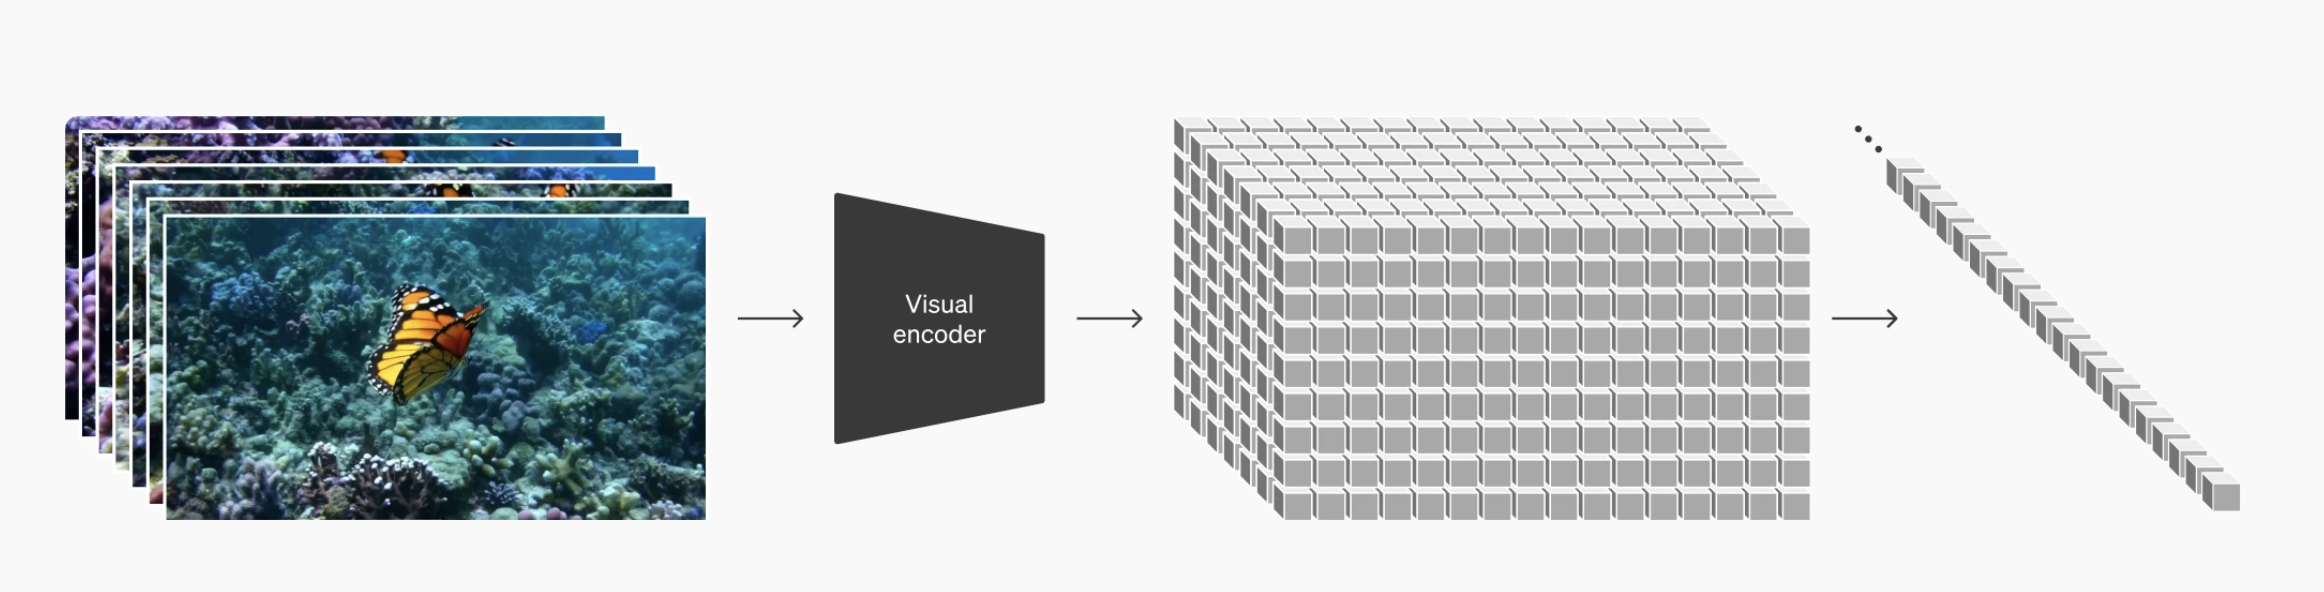
\includegraphics[width=0.8\textwidth]{2.png} 
    \caption{视频切分为Patches} 
    \label{Fig.main2} 
\end{figure}


总的来说,Sora先将视频压缩到低维度的潜在空间,然后再将其分解为空间和时间的视频数据块,也就是Patches。见上图。


而与视频切分处理相关的工作主要引用了ViVi::A Video Vision Transformer这项研究。
这项研究的核心内容就是基于纯Transformer的模型,用于视频分类任务,借鉴了近期图像分类领域中该类模型的成功经验。
这个模型从输入视频中提取时空spatiotemporal tokens,然后通过一系列Transformer层进行编码。关键在于,为了处理视频中遇到的长序列标记,作者提出了几种有效的模型变体,这些变体将输入的空间和时间维度进行了分解。
其中最主要的就是切分策略。

其核心在于采用了分层结构,先对视频的空间信息进行处理,再处理时间信息。
\begin{figure}[h] 
    \centering 
    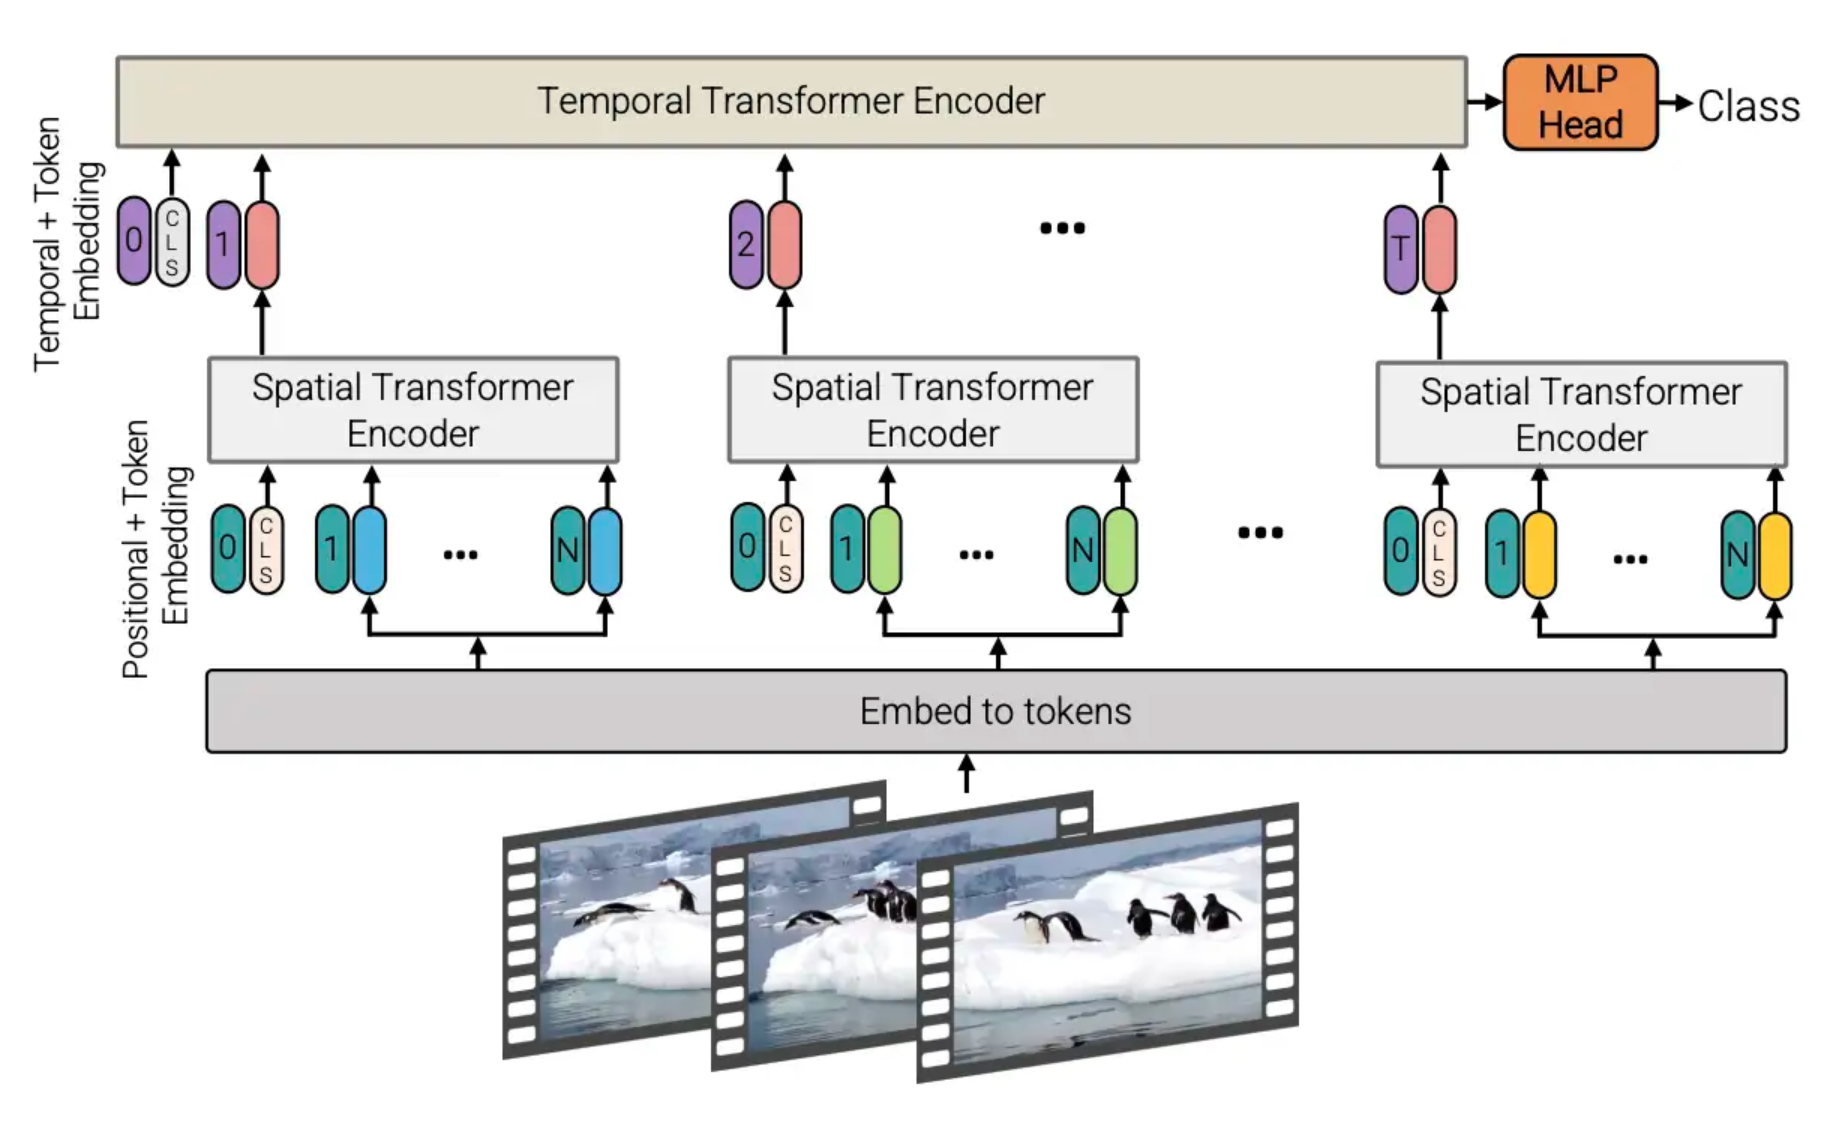
\includegraphics[width=0.8\textwidth]{3.png} 
    \caption{视频切分策略:分层结构} 
    \label{Fig.main3} 
\end{figure}


\begin{figure}[h] 
    \centering 
    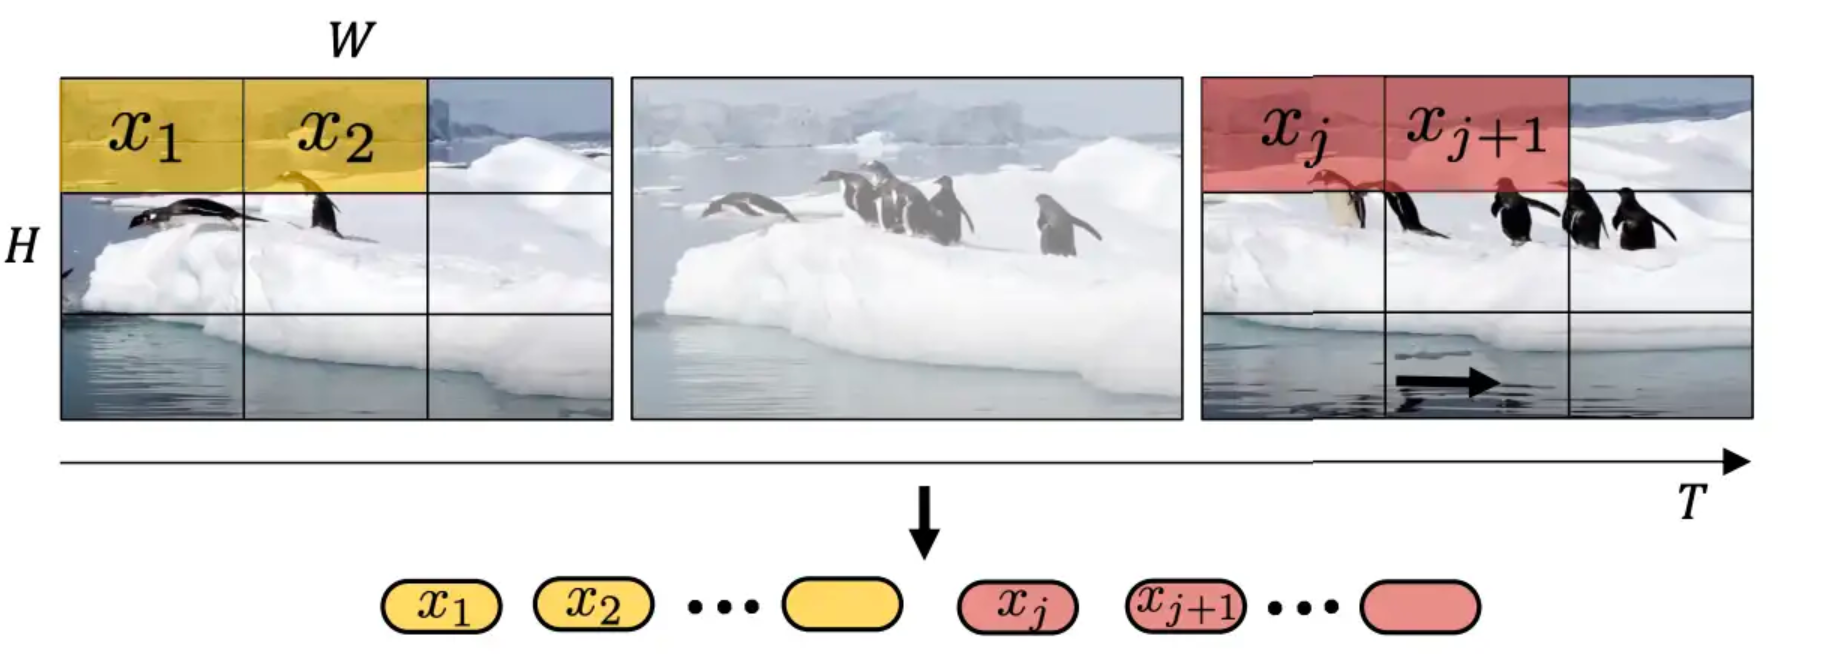
\includegraphics[width=0.8\textwidth]{4.png} 
    \caption{分层结构中的切分} 
    \label{Fig.main4} 
\end{figure}
这种方法相较于传统的直接处理视频序列的方法,更加高效,能够更好地处理长序列标记的问题。
同时使得模型聚集于空间信息的处理,随后再是时间纬度。在提高了处理效率的同时,也保留了关键信息。

虽然增加了模型的数量,但实际的计算量并没有增加,因为时间维度的处理可以采取分层处理。

\subsubsection{分辨率}
Sora给出的技术报告中说到,它可以采用宽屏1920x1080p的分辨率,竖屏1080x1920p的分辨率,以及两者之间的所有尺寸。这让Sora可以直接用不同设备的原生宽高比创建内容。
\begin{figure}[htbp] 
    \centering 
    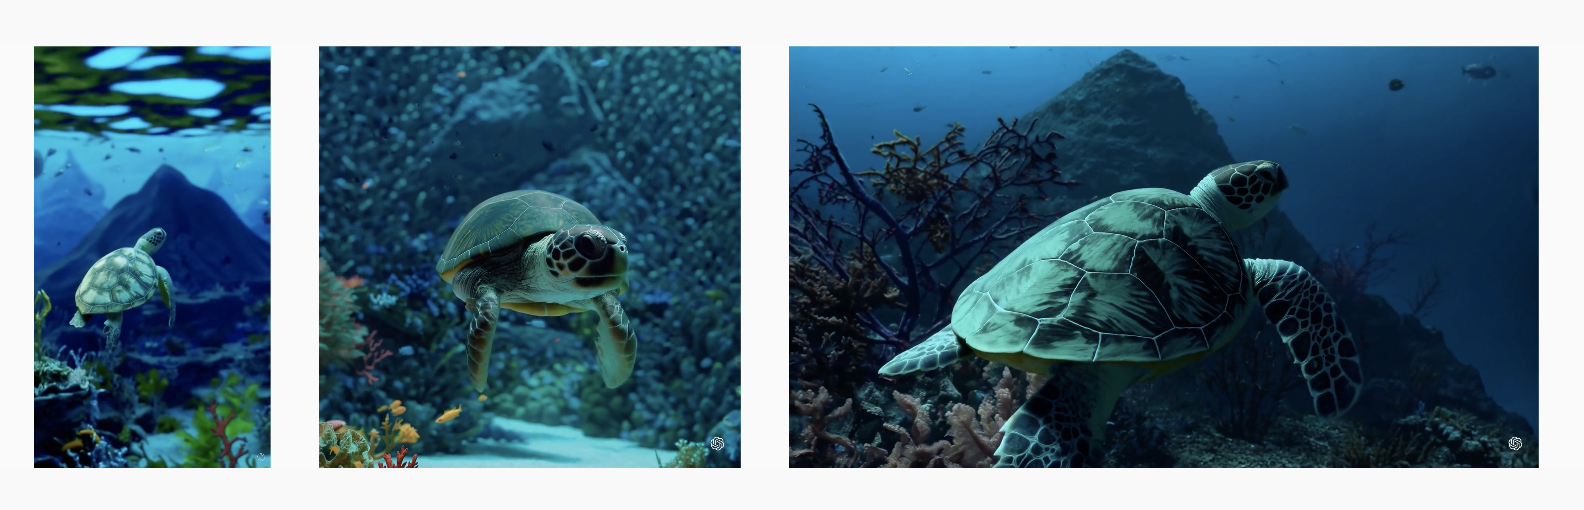
\includegraphics[width=0.8\textwidth]{5.png} 
    \caption{Sora给出的分辨率例子} 
    \label{Fig.main5} 
\end{figure}

而原文也提及和引用了Patch n’ Pack: NaViT, a Vision Transformer for any Aspect Ratio and Resolution》这一研究的核心理念和技术。。
因此,Sora模型可能采用了该研究中的技术,来实现对于输出视频的分辨率灵活变化。

通过打包宽高比的可变分辨率图像,使得Sora减少训练时间,提高性能。
NaViT利用序列打包技术,使得训练时可以处理不同分辨率和宽高比的输入,将不同图像的Patches组合序列,让模型同时处理多个图像片段。
为了防止不同图像之间的交互,还引入了自注意力遮蔽(masked-out),。这种遮蔽可以让模型专注于图像内的相关部分,而不会受到其他图像的影响。
然后重新设计位置嵌入来适应变化的宽高比,同时保留了空间信息。最后得到了结果如图5。
\begin{figure}[htbp] 
    \centering 
    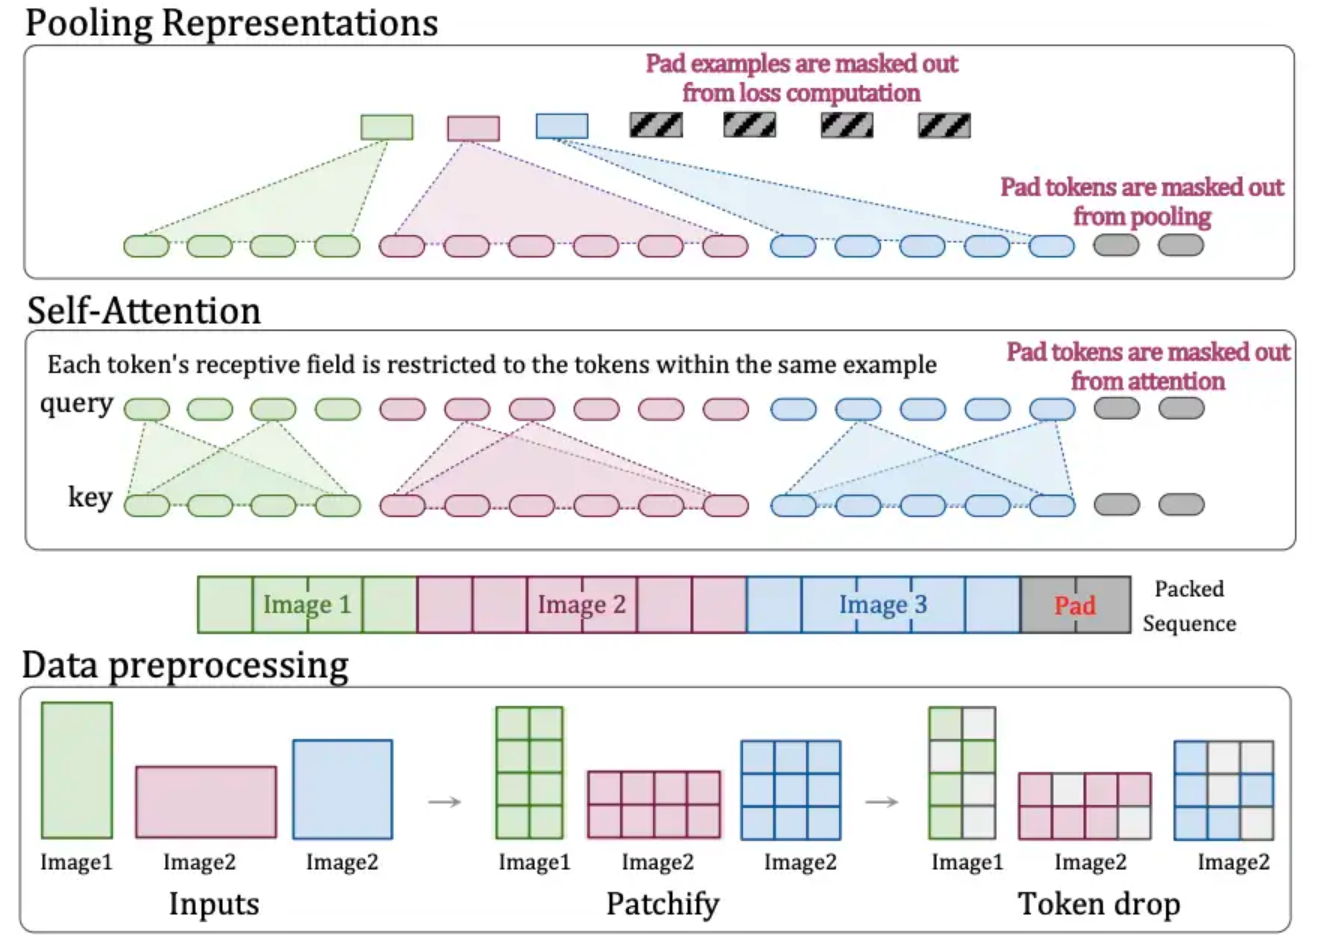
\includegraphics[width=0.505\textwidth]{6.png} 
    \caption{灵活的输入处理} 
    \label{Fig.main6} 
\end{figure}


\section{课程感想}
通过四个老师的课程,我对人工智能有了更加深入的了解。从人工智能的定义、技术分支、前沿技术再到智能机器人,人工智能的发展和应用前景十分广阔。

我明白了什么是人工智能,就是计算机科学加上智能表现所构成的环境交互,制造具有智能表现的机器,能够与环境交互并努力实现目标,就是人工智能。
老师所介绍的Sora也加深了我对人工智能的兴趣。同时,在学习自然语言处理方面,我了解到人工智能在语音识别、文本处理等方面的应用,以及多种领域的实际应用案例。
同时,我也学习了在分析自动驾驶的时候,要多方面去研究,从人、环境、路线、气候、时间等多种方向讨论。
智能机器人在制造业,医疗,军事也有着广泛应用,还有在极端特种情况下也能应用。

通过学习人工智能导论课程,我认识到人工智能的定义,自然语言处理,人工智能汽车,智能机器人等方面知识。同时,我意识到人工智能已经深入到我们生活的方方面面,未来的发展潜力巨大。我对人工智能的前景充满了信心,
也无比期待未来人工智能技术的发展。未来,我会努力学习人工智能的相关知识,为人工智能的发展贡献自己的力量。


感谢本课程的老师,让我对人工智能有了更全面的认识。

\section{参考}
1.https://openai.com/index/video-generation-models-as-world-simulators/

2.https://proceedings.neurips.cc/paper\_files/paper/2023

/hash/06ea400b9b7cfce6428ec27a371632eb-Abstract-Conference.html
\end{document}
